
\subsection{Inleiding}

Wij willen jullie een spel laten maken wat zich afspeelt in een enorm grote arena, met veel publiek die veel geld betaald hebben om naar dit schouwspel te komen kijken. In deze arena zijn verschillende robots op zoek naar hun eigen thuisvak.

\subsection{Spelregels}

Het spel wordt in de arena gespeeld, waarin een vooraf gedefinieerd eindig spelbord aanwezig is.
Er zijn twee type robots die aan het spel deelnemen. Het eerste type robot kan zich in iedere richting (boven, onder, rechts of links) precies een vakje verplaatsen. Het tweede type robot kan twee soorten zetten doen. De robot kan 1, 2 of 3 hokjes vooruit lopen, of de robot kan draaien, waarbij hij 90, 180 of 270 graden draait. Dit tweede type kan dus in een beurt lopen of draaien, echter niet beide.\\
Er zijn verder vijf type vakjes.
\begin{enumerate}
  \item thuisvakken, als een robot op zijn eigen thuisvak komt heeft hij gewonnen.
  \item hintvakken, als een robot hierop komt krijgt hij een hint waar zijn thuisvak is.
  \item lopende banden, dit zijn vakken waarbij de robot verplaatst wordt, zodra hij hier op staat. Deze lopende banden gaan met een oneindige snelheid, dus zodra een robot op een lopende band stapt wordt hij verplaatst naar een andere plek, voordat hij zelf om een nieuwe verplaatsing kan vragen.
  \item bezette vakken, dit zijn vakken waar al een andere robot staat. Dit kan ook een defecte robot zijn.
  \item normale vakken, dit zijn vakjes waarbij er niets speciaals gebeurt.
\end{enumerate}

\noindent Alle robots in het speelveld zijn op zoek naar hun eigen thuisvak. Iedere robot heeft precies \'{e}\'{e}n thuisvak. Om de robots hierbij een beetje te helpen, zijn er ook verschillende hintvakken, zie figuur 1, (ook hiervan weet de robot de locatie niet, hij moet dus maar met geluk op een hintvak terecht komen).\\
Zodra een robot op een hintvak terecht komt, krijgt de robot een hint over de richting te volgen naar zijn thuisvak. Een hint bestaat puur en alleen uit een richting waar het thuisvak zich bevindt (boven, onder, rechts of links). Als eenzelfde robot een tweede maal op een hintvak terecht komt, kan hij een andere hint krijgen dan de eerste keer.

\begin{figure}
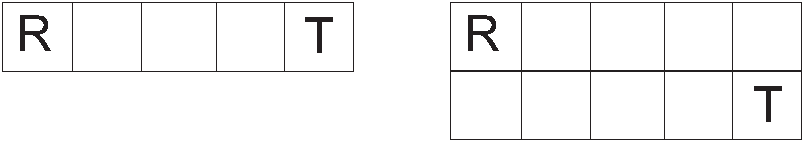
\includegraphics{informal/plaatjes.pdf}
\caption{De robot R staat op een hintvak, en T is het thuisvak. Twee situaties: In de situatie links is de hint $"$rechts$"$. In de situatie rechts zijn er meerdere mogelijkheden, $"$onder$"$, $"$rechts$"$ of $"$rechts en onder$"$.}
\label{hintvakken}
\end{figure}

De locatie van de hintvakken en van de thuisvakken is statisch. Een robot kan hierover dus informatie opslaan. De robot kan geen gegevens over zijn eigen locatie opslaan, aangezien er ook rotatie-transportbanden op het speelveld aanwezig zijn. Iedere transportband verplaatst een robot naar een willekeurige plaats. De robot kan tijdens het transport ook geroteerd zijn. Daarom zijn het ook rotatie-transportbanden. De robot kan dus geen gegevens bewaren over zijn locatie, aangezien de robot verplaatst kan zijn tussen twee beurten. De robots kunnen de transportbanden niet zien. Ze merken door hun ingebouwde gyroscopen wel dat ze bewogen zijn, de gyroscopen zijn echter niet goed genoeg om bij te kunnen houden in welke richting de robot verplaatst is.\\
Zodra een robot op zijn thuisvak aangekomen is, heeft deze robot gewonnen, en kan hij alle andere robots laten ontploffen. Het einde, het ontploffen van alle verliezende robots, is het spektakel waarvoor het publiek gekomen is. Ze barsten na het ontploffen dan ook in juichen uit.

\subsection{Spelbord}

Er is een bord, zodat bijgehouden kan worden welke robot waar staat. Dit bord houdt bij welke robot op welke positie staat. Opdat de spelers met het bord kunnen communiceren moet er een controller zijn. De communicatie geschiedt alleen op de volgende volgorde: het bord ontvangt een request van de speler via de controller. Het bord antwoordt de controller. Deze zal dan weer de speler informeren.\\
Omdat de schoonmakers een beetje lui zijn, staan er op het veld nog kapotte robots uit de vorige gevechten. Het aantal kapotte robots kan vari\"{e}ren van 10 tot 20 procent van het totaal aantal vakjes. Als een robot een verzoek indient om naar een van deze vakjes te gaan, of naar een van de vakjes waarop een andere robot staat, dan wordt dit verzoek afgewezen omdat dit vakje dan al bezet is.\\
Iedere keer dat het spelbord een request toestaat, kiest het bord ook twee vakjes welke omgewisseld worden, als hier een (defecte) robot op staat of als hier een lopende band is, worden de robot en/of lopende band mee verplaatst. Dit houdt in dat ook de ori\"{e}ntatie van de speler en de lopende band verandert kan zijn. Het bord dient er echter wel voor te zorgen dat het altijd mogelijk blijft voor iedere robot om zijn thuisvak te halen. Het bord kan hier alle type vakjes, behalve de hint en thuisvakken verplaatsen. De robot kan dus alleen hier informatie over bijhouden.\\
Als een robot verplaatst wordt, door een lopende band, of doordat er twee vakjes verwisseld worden, geeft het bord dit door aan de controller, die het weer door zal geven aan de robot.\\
Het bord keurt alle zetten af zolang het nog niet ge\"{\i}nitialiseerd is.

\subsection{Speler}

Een speler is een robot die mee doet aan het spelletje. Als de speler zich wil verplaatsen stuurt hij een verzoek tot verplaatsing naar de controller. Het bord krijgt een request van de speler via de controller. Het bord zal beslissen of de zet legitiem is of niet, zo ja dan wordt de speler verplaatst. Aan de controller wordt terug gegeven of de robot is verplaatst of niet, die dit op zijn beurt weer terug geeft aan de speler. \\
Indien een speler op een lopende band komt, maar het einde van de lopende band is geblokkeerd door een andere mogelijk defecte robot, zal de robot op het laatste stukje van de lopende band blijven staan. En kan hij hier wel weer afstappen, als de nieuwe plek tenminste niet ook geblokkeerd is.\\
De spelers kunnen hun zetten gelijktijdig doen, er wordt dus geen volgorde afgedwongen.

\subsection{Viewer}

Om het publiek een beter zicht op het spel te geven hangen er op verschillende plaatsen in de arena beeldschermen. Deze beeldschermen geven een visuele representatie van de staat van de controller en dus ook het bord.

\subsection{Use-Case Scenario's}
Hieronder staan een aantal Use-Cases, zodat jullie kunnen zien hoe de communicatie tijdens het spel verloopt.
\subsubsection*{Robot wil verplaatsen}
\begin{description}
  \item[Pre:] True.
  \item[Trigger:] Robot vraagt toestemming om een stap te doen.
  \item[Guarantee:] Robot is verplaatst.
  \item[Scenario]
    \begin{description}
        \item[]
        \item[Main]
            \begin{enumerate}
              \item[]
              \item De robot zegt tegen de controller dat hij wil verplaatsen.
              \item Controller geeft vraag door aan het bord.
              \item Het bord keurt de vraag goed en verplaatst de robot.
              \item Controller geeft door dat hij verplaatst is.
            \end{enumerate}
        \item[Alternative]
            \begin{itemize}
                \item[]
                \item[3] Het bord keurt de vraag af en de robot blijft staan.
                \item[4] Controller geeft door dat de robot geen toestemming heeft.
            \end{itemize}
    \end{description}
\end{description}
\newpage
\subsubsection*{Robot stapt op lopende band}
\begin{description}
  \item[Pre:] Stap is toegestaan.
  \item[Trigger:] Vakje waar robot op komt is een lopende band.
  \item[Guarantee:] Robot is verplaatst over lopende band.
  \item[Scenario]
    \begin{description}
        \item[]
        \item[Main]
            \begin{enumerate}
              \item[]
              \item Robot stapt op lopende band.
              \item Robot eindigt op vakje na de lopende band.
              \item Robot krijgt te horen dat hij verplaatst is.
            \end{enumerate}
    \end{description}
\end{description}

\subsubsection*{Robot stapt op hintvak}
\begin{description}
  \item[Pre:] Stap is toegestaan.
  \item[Trigger:] Robot komt op een hintvak terecht.
  \item[Guarantee:] Robot krijgt een hint over de positie van zijn thuisvak.
  \item[Scenario]
    \begin{description}
        \item[]
        \item[Main]
            \begin{enumerate}
              \item[]
              \item Robot stapt op hintvak.
              \item Het bord bepaalt aan de hand van de relatieve positie van het thuisvak t.o.v de robot, de hint.
              \item De hint wordt via de controller doorgegeven aan de robot.
            \end{enumerate}
    \end{description}
\end{description}

\subsubsection*{Robot stapt op thuisvak}
\begin{description}
  \item[Pre:] Stap is toegestaan.
  \item[Trigger:] Robot stapt op thuisvak.
  \item[Guarantee:] De verplaatste robot heeft gewonnen.
  \item[Scenario]
    \begin{description}
        \item[]
        \item[Main]
            \begin{enumerate}
              \item[]
              \item Robot stapt op het thuisvak.
	          \item Het bord laat Spelers weten dat de verplaatste robot heeft gewonnen.
            \end{enumerate}
    \end{description}
\end{description}
\newpage
\subsubsection*{Vakjes worden gewisseld}
\begin{description}
  \item[Pre:] True.
  \item[Trigger:] Het bord heeft de request van de robot goedgekeurd.
  \item[Guarantee:] Na het verwisselen van de twee vakjes moet er een mogelijkheid zijn voor alle robots om het thuisvak te kunnen bereiken.
  \item[Scenario]
    \begin{description}
        \item[Main]
            \begin{enumerate}
              \item[]
              \item Er worden twee geldige vakjes gekozen.
              \item De vakjes worden gewisseld.
            \end{enumerate}
        \item[Alternative]
            	\begin{itemize}
			     \item[]
                 \item[2] Als er op een of beide vakjes een lopende band en/of een robot aanwezig is, dan worden alle robots en lopende banden op deze twee vakjes willekeurig een richting op gedraaid (de richting voor en na het draaien kan hetzelfde zijn).
			     \item[3] Het bord geeft via de controller door aan de speler dat de robot verplaatst is.
            	\end{itemize}
    \end{description}
\end{description}
